%narms.tex, an example driver file for Balkema documents.

%use the following for A4 paper:
\documentclass[12pt,a4paper,twocolumn,fleqn]{narms}

% packages needed
\usepackage{subfigure}
\usepackage{epsfig}
\usepackage{timesmt}

% add here more packages based on the document format
\usepackage{xcolor}


% setting math equation indent from left 0pts

\mathindent=0pt%

% use this for chicaco style reference
% Author references
% IMPORTANT: Author wants to format references in chicaco style Author must use BiBTex
% IMPORTANT: Author wants to format numbered references remove chicaco style file and \bibliographystyle{chicaco}

%\usepackage{chicaco}

%  \cite{key}
%    which produces citations with full author list and year.
%    eg. (Brown 1978; Jarke, Turner, Stohl, et al. 1985)

%  \citeNP{key}
%    which produces citations with full author list and year, but without
%    enclosing parentheses:
%    eg. Brown 1978; Jarke, Turner & Stohl 1985

%  \citeA{key}
%    which produces citations with only the full author list.
%    eg. (Brown; Jarke, Turner & Stohl)

%  \citeANP{key}
%    which produces citations with only the full author list, without
%    parentheses eg. Brown; Jarke, Turner & Stohl

%  \citeN{key}
%    which produces citations with the full author list and year, but
%    can be used as nouns in a sentence; no parentheses appear around
%    the author names, but only around the year.
%      eg. Shneiderman (1978) states that......
%    \citeN should only be used for a single citation.

%  \shortcite{key}
%    which produces citations with abbreviated author list and year.

%  \shortciteNP{key}
%    which produces citations with abbreviated author list and year.

%  \shortciteA{key}
%    which produces only the abbreviated author list.

%  \shortciteANP{key}
%    which produces only the abbreviated author list.

%  \shortciteN{key}
%    which produces the abbreviated author list and year, with only the
%    year in parentheses. Use with only one citation.

%  \citeyear{key}
%    which produces the year information only, within parentheses.

%  \citeyearNP{key}
%    which produces the year information only.


%%%%%%%%%%%%%%%%%%%%%%%%%%%%%%%%%%%%%%%%%%%%%%%%%%%%%%%%%%%%%%%%%%%
%%%  All this stuff is from modifying the article.cls for Balkema
%%%  specifications.

%\title{...}
%\author{...}
%use \aff for author affiliations
% use \authornext for from second author
% empty line space between multiple authors
%\abstract{...}
%\maketitle{}

%%%%%%% Style for TABLES
% insert tabular command inside \tabletext{} this will produce tables in 10pts

\begin{document}
\title{Fast early flood warning systems exploiting catchment specific behavior}
\author{{S. Rusca} \\
{\aff{ETH Zurich, Switzerland}} \\\\
{\authornext{J. P. Carbajal}}\\
{\aff{University of ???}}
%{\authornext{R. Schielen}}\\
%{\aff{Department of Water Engineering and Management}} \\
%{\aff{University of Twente, Enschede, The Netherlands.}}\\
} \maketitle


\section*{Abstract}

Floods due to heavy rain are among the most destructive events in hydrology. 
Numerical models cannot directly be used for real time flood prediction due to
their high complexity. Ad hoc surrogate models provide great speed
ups with minor accuracy losses.


\section{Introduction}

In this work, we present a methodology for developing a surrogate model of
a detailed (non-linear shallow water equations) simulator. The simulator used
for this scope is \textit{FullSWOF\textunderscore2D-v.1.07.00}
\cite{noauthor_fullswof_nodate}. The performance of the resulting emulator-based
early flood warning system tailored for the catchment in question is discussed
and analyzed.\\

An early warning system has to be understood as one capable of giving within
seconds a prediction of whether based on current conditions (soil moisture content,
potential infiltration, \dots) and meteorological forecast an occurring rain
event will result in major flooding or not, and if yes within how much time.\\

Fine tuned physically based simulators are able
to produce trustworthy flood predictions but are unusable as early warning
systems due to their high computational cost.
Fast surrogate models based on these simulators can yield results of the same
order of accuracy with speed-up factors of up to $10^6$.
\textcolor{red}{reference of same idea in volcanology}


\section{Methodology}

A synthetic squared catchment of size 2km x 2km was generated in order to
perform the simulations. Simulations were run to obtain response hydrographs of
the given catchment to different rain events and soil saturation conditions.
In particular the parameters initial soil saturation and rain intensity were
varied. A constant rain with a duration of 6\,h was chosen, while a longer
duration was set for the simulation, in order to be able to observe the
hydrograph recession.

\begin{figure}[t]
  \centering
  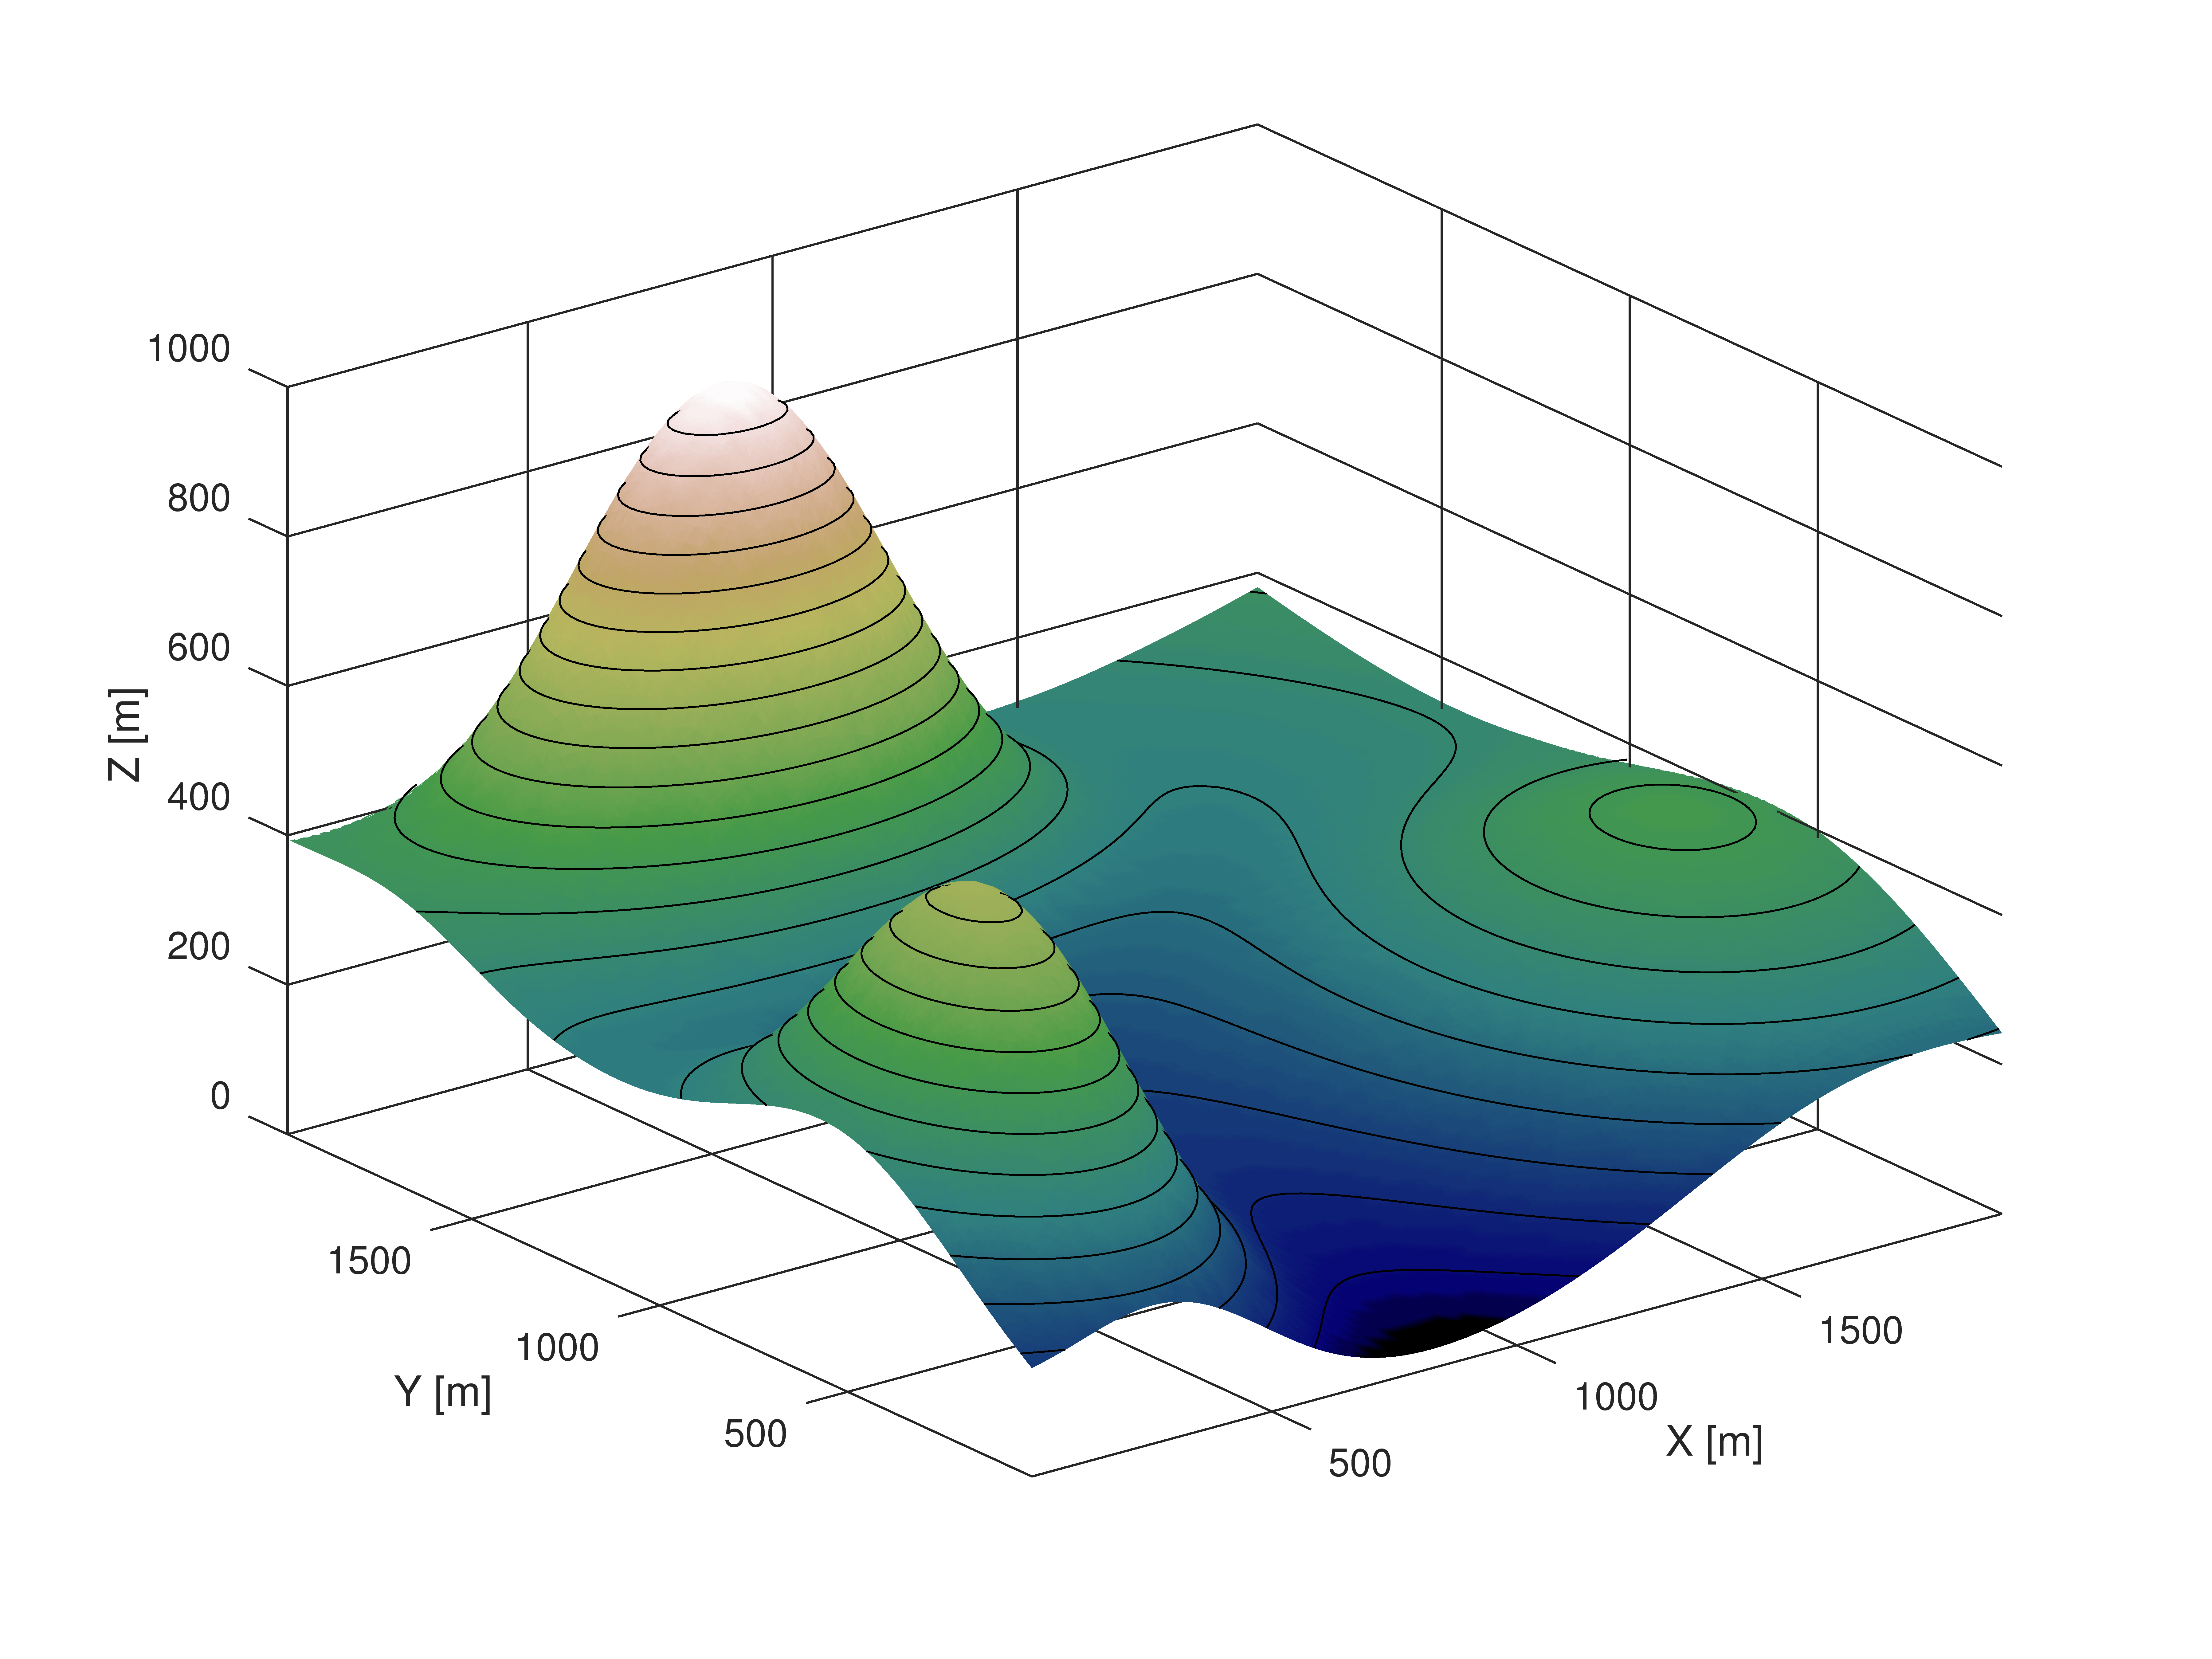
\includegraphics[width=0.4\textwidth]{img/topography.png}
  \caption{Synthetic topography produced in \textit{Octave} \cite{noauthor_gnu_nodate}}
  \label{img:topography}
\end{figure}

Figure \ref{img:topography} here above shows the synthetic topography used.
50 simulations were run with soil initial saturations in a range of $[0 - 1]$
and rain intensities in a range of $[10 - 35]\,mm/h$.\\

As output response the total outflow through the catchment bottom boundary was used.
This is represented in the hydrographs of Figure \ref{img:hydrographs}.

\begin{figure}[t]
  \centering
  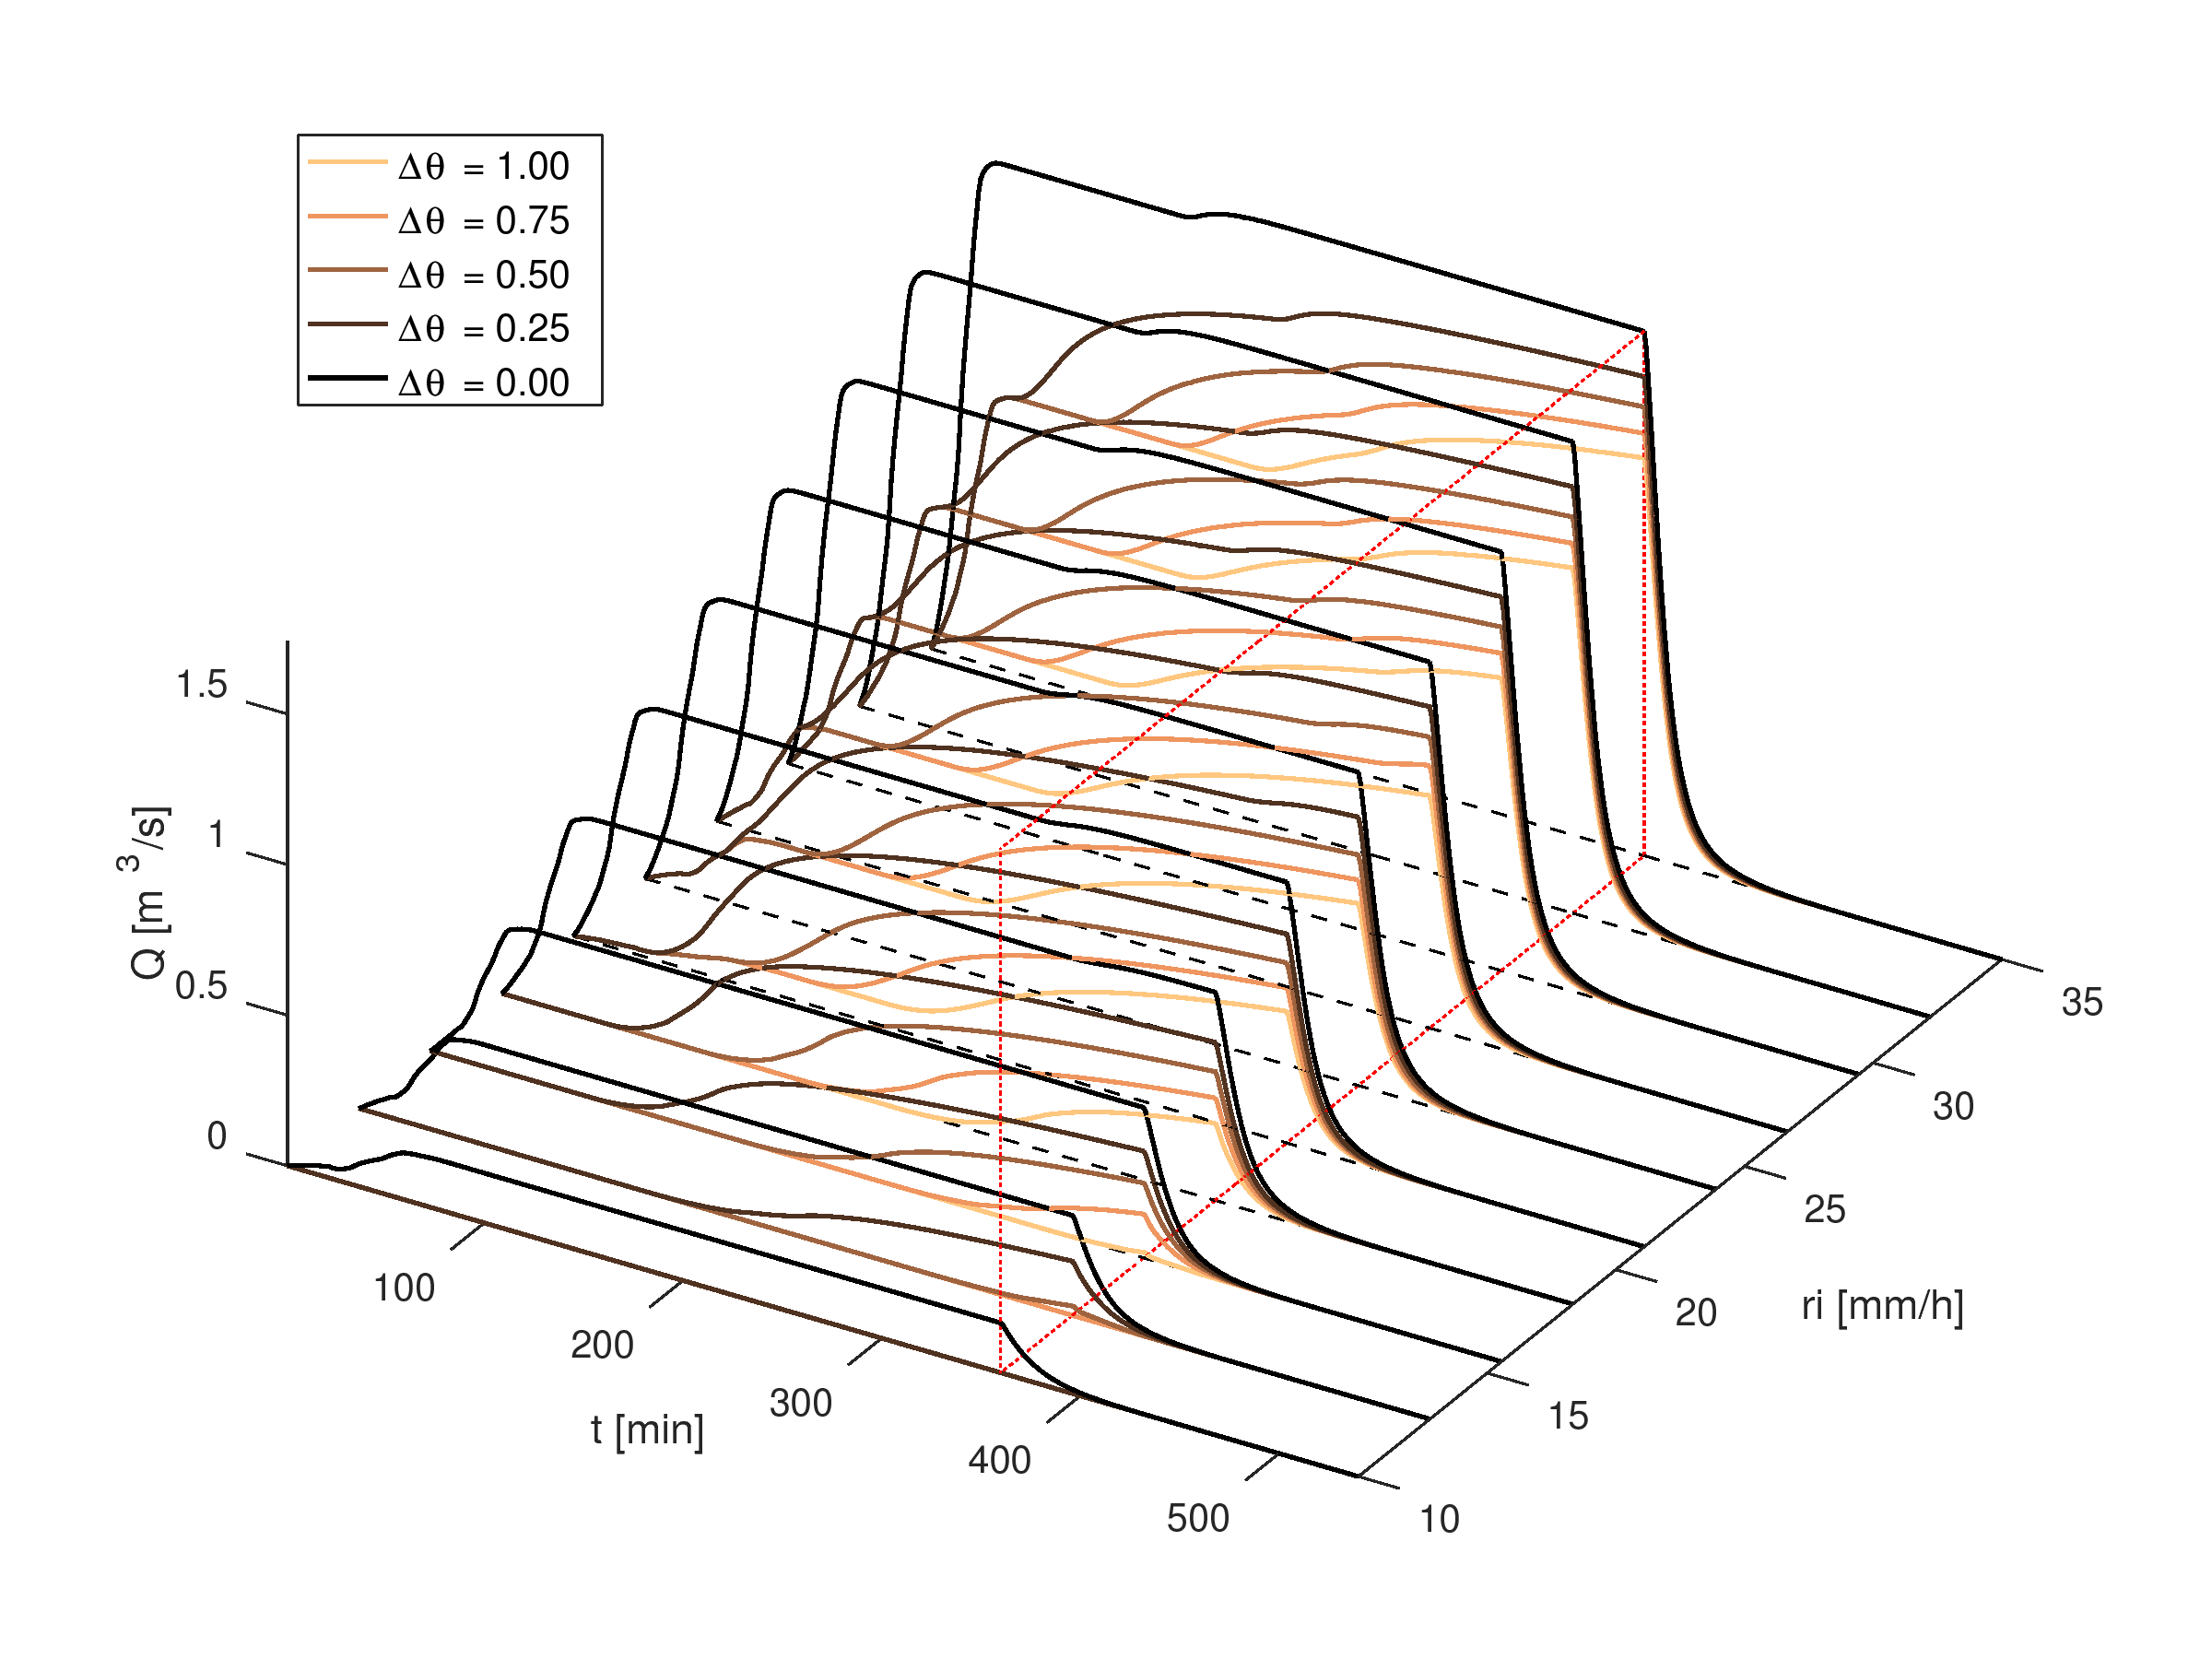
\includegraphics[width=0.4\textwidth]{img/hydrographs3d.png}
  \caption{Response hydrographs of the catchment to the different rain events}
  \label{img:hydrographs}
\end{figure}

The hydrographs show different responses depending on
the soil initial saturation and the rain intensity which was applied.
In some cases, in particular by heavy rain and high initial soil
saturation values, the appearance of surface runoff is very rapid.
In other cases this just happens after it has rained for hours or
does not happen at all. The emulator we aim to build should be used as
an early flood warning system. The variable which it is trying to predict is
then the time at which a certain $Q_{thhold}$, the maximum discharge for which the
various hydraulic structure on the channel downstream of the catchment were
dimensioned, is reached. As observable from the hydrographs this time can be
very variable depending on the value of $Q_{thhold}$ or can never be reached.



\section{Acknowledge}

Here you can insert acknowledge.

\bibliography{ref}
\bibliographystyle{plain}



\end{document}
